\documentclass{article}

\usepackage{fancyhdr}
\usepackage{setspace}
\usepackage{titlesec}
\usepackage{tocloft}
\usepackage{lipsum}
\usepackage[fleqn]{amsmath}
\usepackage{amssymb}
\usepackage{hyperref}
\usepackage{url}
\usepackage{graphicx}
\usepackage{geometry}
\usepackage{enumitem}
\usepackage{parskip}
\usepackage{chemfig}
\usepackage{pdfpages}
\usepackage{tikz}
\usepackage{fancybox}
\usepackage{makecell}
\usepackage{pgfplots}
\usepackage{soul}
\usepackage{multirow}
\usepackage{ulem}
\usepackage{wrapfig}
\usepackage{subcaption}
\usepackage[T1]{fontenc}
\usepackage{esvect}
\usepackage{xcolor}
\usepackage{booktabs}
\usepackage{array}
\usepackage{colortbl}
\usepackage{fontspec}
\usepackage{tabularx}
\usetikzlibrary{arrows}
\usetikzlibrary{decorations.pathreplacing}
\pgfplotsset{compat=1.17}
\definecolor{darkgreen}{RGB}{0, 160, 0}

\geometry{
    a4paper,
    total={170mm, 257mm},   
    left=20mm,
    top=20mm
}   

\hypersetup{
    colorlinks=true,
    linkcolor=black,
    urlcolor=blue,
    pdftitle={Team 31_Review 3 HS24}
}

\pagestyle{fancy}
\fancyhf{}
\fancyhead[L]{\leftmark}
\fancyhead[R]{\thepage}
\renewcommand{\headrulewidth}{0.4pt}

% === BIBLIOGRAPHY ===
\usepackage[utf8]{inputenc}
\usepackage{csquotes}
\usepackage[style=apa, backend=biber, doi=true, url=true]{biblatex}
\addbibresource{ref.bib}
\DeclareFieldFormat[article]{volume}{\textbf{#1}}
\DeclareFieldFormat[article]{journaltitle}{\textit{#1}}
% ====================

\newcommand{\figbox}[1]{ 
    \begin{figure*}[ht!]        
        \begin{center}            
            \fbox{#1}        
        \end{center}    
    \end{figure*}
}

\newcommand{\wrapfill}{
    \par
    \ifnum \value{WF@wrappedlines} > 0
        \addtocounter{WF@wrappedlines}{-1}%
        \null\vspace{
            \arabic{WF@wrappedlines}
            \baselineskip
        }
        \WFclear
    \fi
    \phantom{}
}

\newcommand{\difference}{\,\backslash\,}
\newcommand{\rem}{\underline{Remark}: }
\newcommand{\nots}{\underline{Notation}: }
\newcommand{\prf}{\underline{Proof}: }
\newcommand{\exs}{\underline{Example}: }
\newcommand{\defs}{\underline{Definition}: }
\newcommand{\wrn}{\underline{Warning}: }
\newcommand{\sht}{\ |\ }
\newcommand{\pph}[1]{\paragraph{#1} \phantom{}\\}
\newcommand{\dm}{\displaystyle}
\newcommand{\rad}{^{\mathrm{c}}}
\newcommand{\myc}{My$_{\text{celium}}$Tent}

\titleformat{\chapter}[block]{\bfseries\Large}{\thechapter.}{1em}{}

\definecolor{newgreen}{HTML}{4da833}
\definecolor{neworange}{HTML}{e96d2f}
\definecolor{newblue}{HTML}{145d80}

%========= TEXT ===========

\begin{document}

\hypersetup{citecolor=black}

\begin{titlepage}
    \begin{wrapfigure}{l}{7.5cm}
        \hspace*{.01cm}
        
\includegraphics[width=.3\textwidth]{media/hslu-logo-2.png}

        \vspace*{.01cm}
        \hspace*{.16cm}
\includegraphics[width=0.4\textwidth]{media/hslu-svg-logo.png}
    \end{wrapfigure}

    \phantom{}
    \vspace*{-1cm}

    \begin{flushright}
        
\includegraphics[width=.3\textwidth]{media/mytent_logo.jpeg}
    \end{flushright}

    \wrapfill

    \vspace*{-3.5cm}
    {\huge \textbf{Project Context 1}}

    {\Large Final Report}

    \vspace*{3cm}
    \begin{center}
        {\Huge \textbf{My$_{\text{celium}}$Tent}}

        \vspace*{.1cm}
        \textbf{\large The biodegradable tent}
    \end{center}

    \vfill
    {\Large \textbf{Team 31}}\\
    {\large \vspace*{.01cm}
        Althaus Simon\\
        \vspace*{.01cm}
        Berner Nic\\
        \vspace*{.01cm}   
        Frongillo Matteo\\
        \vspace*{.01cm}
        McCarthy Benjamin\\
        \vspace*{.01cm}
        Nyamdorj Narandavaa\\
        \vspace*{.01cm}
    }
    
    \vspace{1cm}
    {\large Horw, 11th December 2024}
\end{titlepage}

\tableofcontents
\thispagestyle{empty}

\vfill
\section{Introduction}

\newpage

\section{Background}

\newpage

\section{Development of concept}
This chapter describes the development of the concept of \myc.
The user scenario is presented at the beginning. From it, a catalogue
of requirements is made, and the result of this chapter is the
concept for the final product.

\subsection{User scenario}
This sub-section explains the primary use case of \myc\ and what describes the
problem it is going to solve. 

\subsubsection{Problem}
Many festival-goers buy cheap, disposable tents with the intent to use them only once.
These tents are often left behind after the event, as they are difficult to carry back,
especially if they are damaged. Because festivals can be rough on tents, people are
reluctant to bring high-quality ones and instead opt for cheap alternatives. As a result,
thousands of plastic and nylon tents are abandoned after major festivals, creating an
environmental issue with large amounts of non-biodegradable waste.

\subsubsection{Objective}
The \myc\ is a biodegradable and recyclable tent made from mushroom roots, designed
as an eco-friendly alternative to single-use plastic tents often abandoned at festivals
and outdoor events. Lightweight, easy to carry, and affordable, it provides a durable yet
temporary shelter that helps reduce plastic waste and minimize environmental impact,
offering festival-goers a sustainable way to enjoy their experience without contributing
to pollution.

\subsection{Requirements catalogue}
Based on the final user scenario and the feedback of potential customers, the requirements
have been defined in the catalogue of requirements (\autoref{tab:cat_of_req}).

\begin{table}[ht!]
    \centering
    \caption{Catalogue of requirements}
    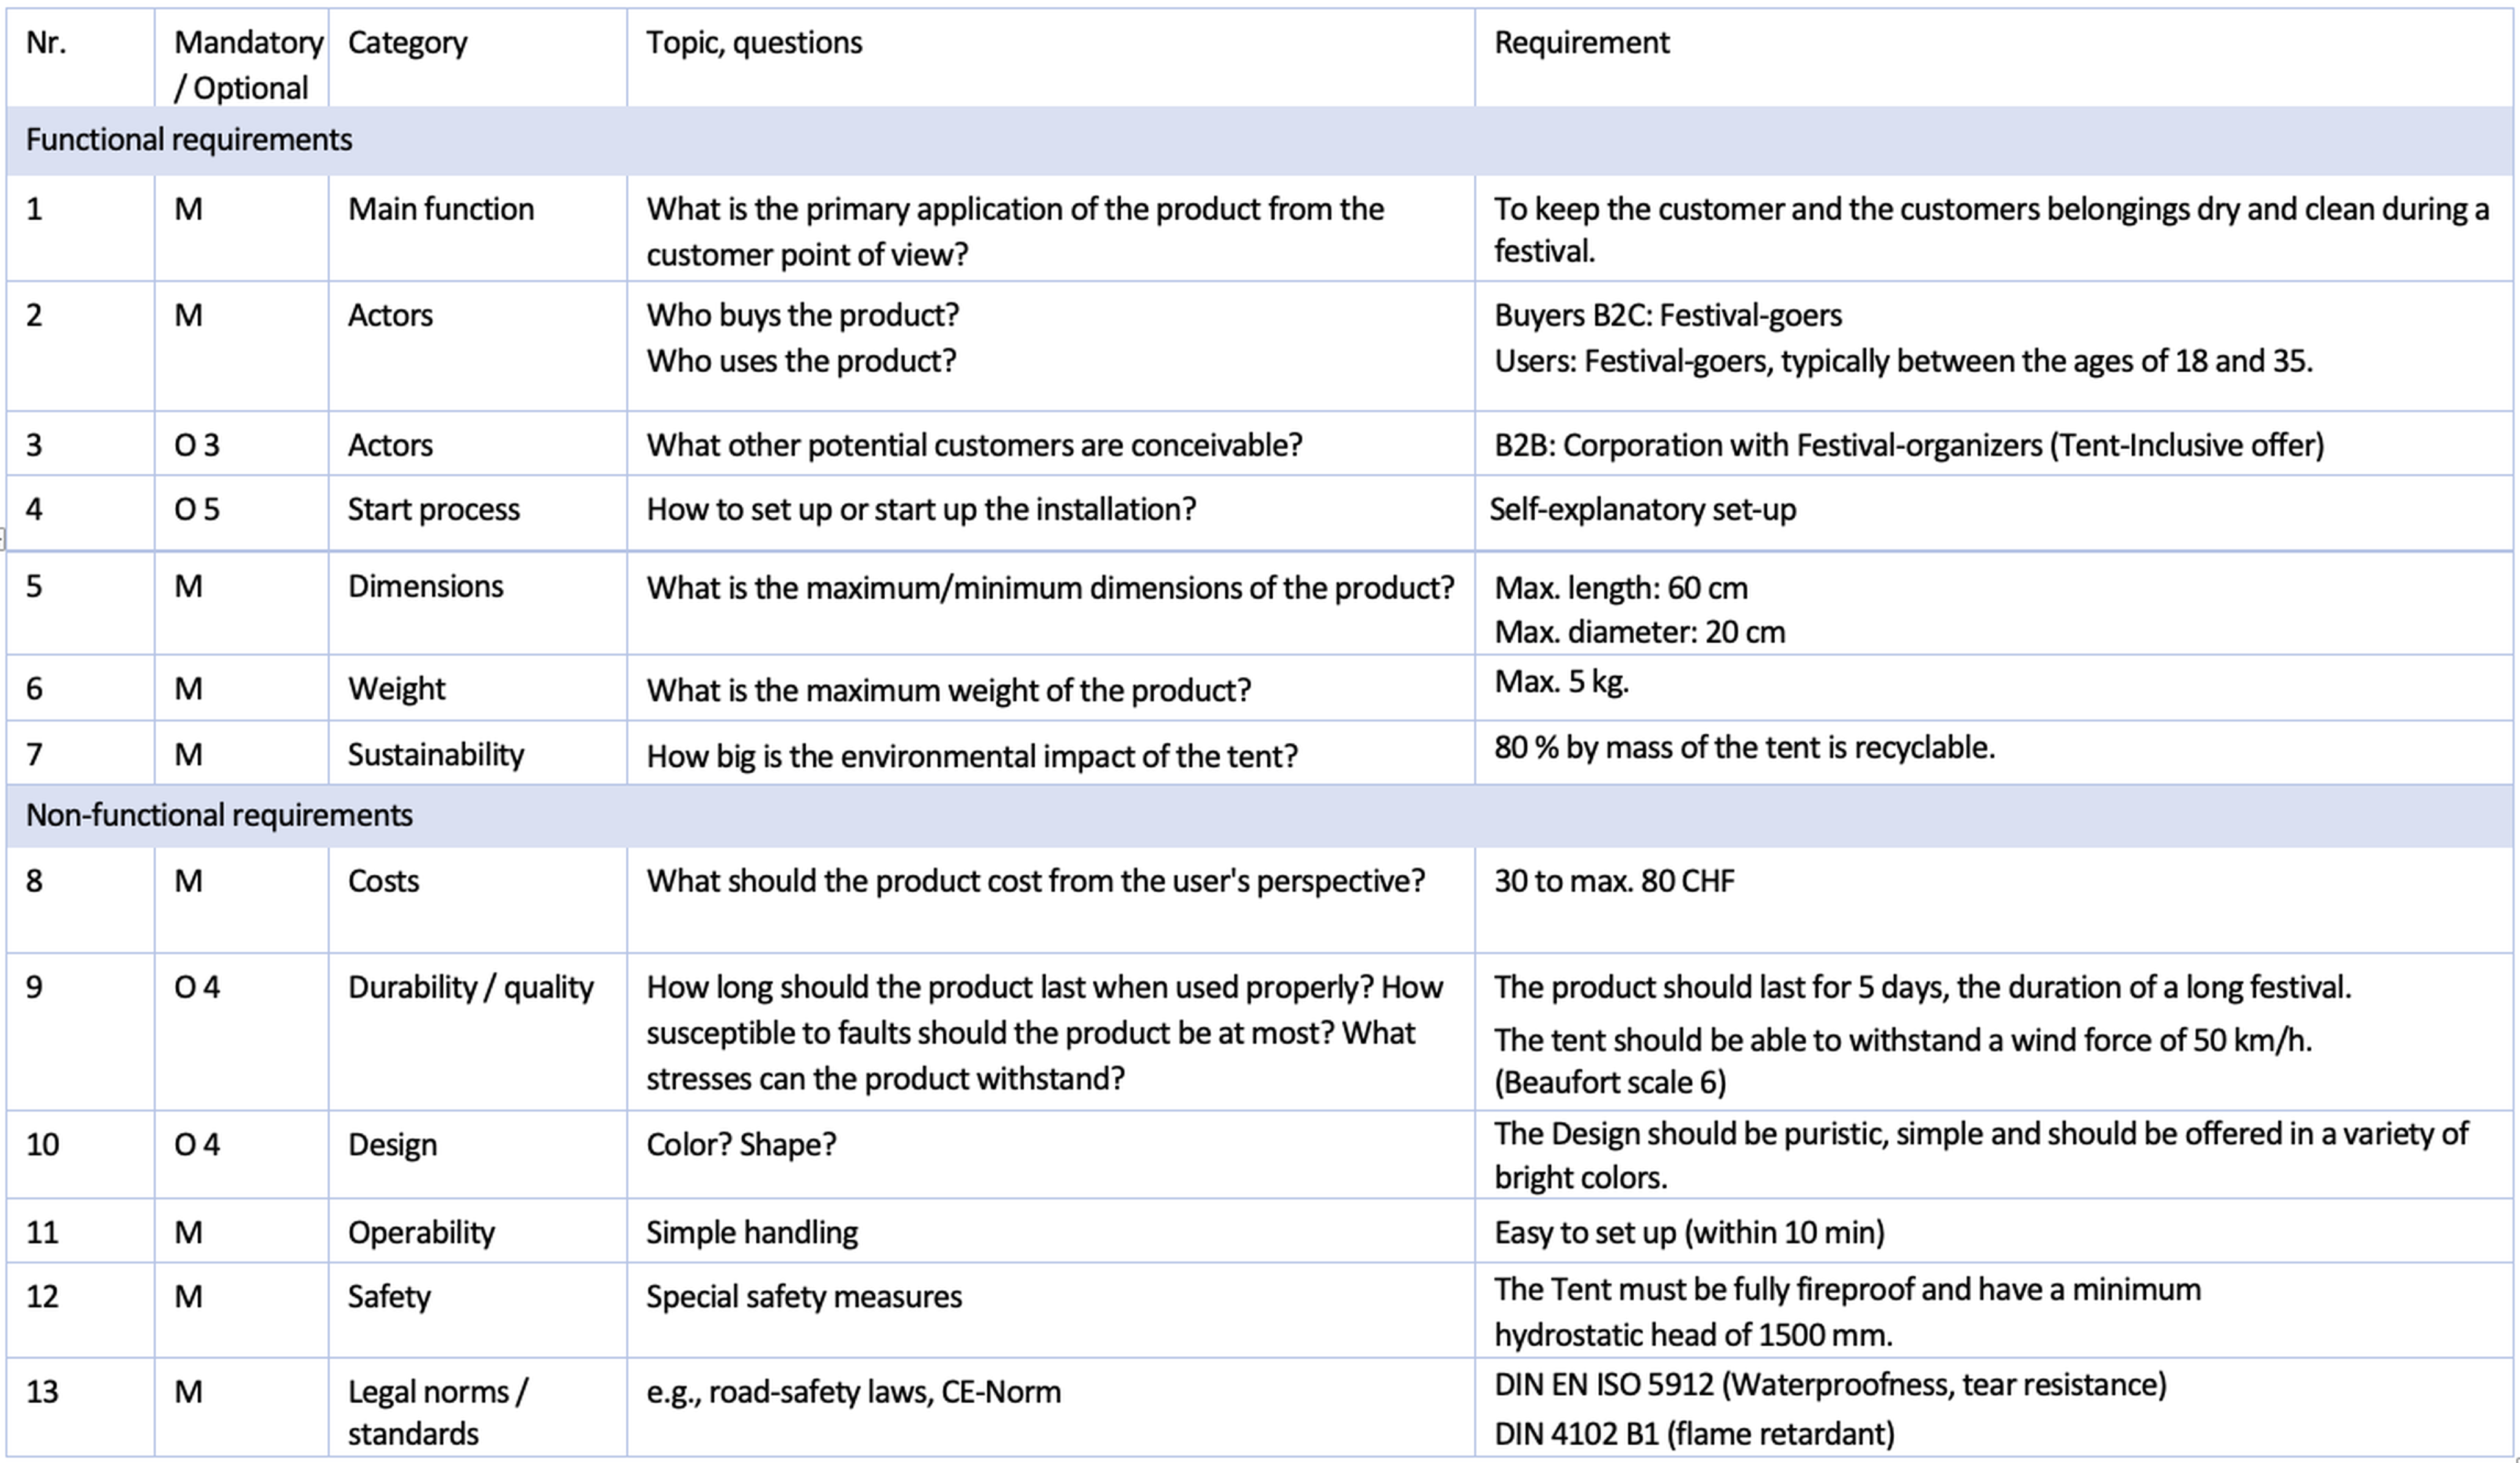
\includegraphics[width=\textwidth]{media/req_cat_high_res.png}
    \label{tab:cat_of_req}
\end{table}

\subsection{Morphological box}
This chapter describes the process of developing three design variants for a biodegradable
festival tent using the morphological box method. The product was divided into key
subproblems, such as shape, size, structure support, lifespan, and material processing.
For each subproblem, a range of possible solutions was researched, resulting in the
initial morphological box ({\color{red}{see Appendix, Table xy}}).

To streamline the process, less critical subfunctions, like color design and biodegradation
duration, were excluded, and unsuitable materials, such as unprocessed Mycelium-Based
Composites (MBCs) and plastic, were removed. The refined morphological box
({\color{red}{see Appendix, Table xy}}) formed the foundation for selecting three
promising design variants, which are detailed in \autoref{tab:morph_box} and the following
section. 

\begin{table}[ht!]
    \centering
    \caption{Morphological box with three solution variants}
    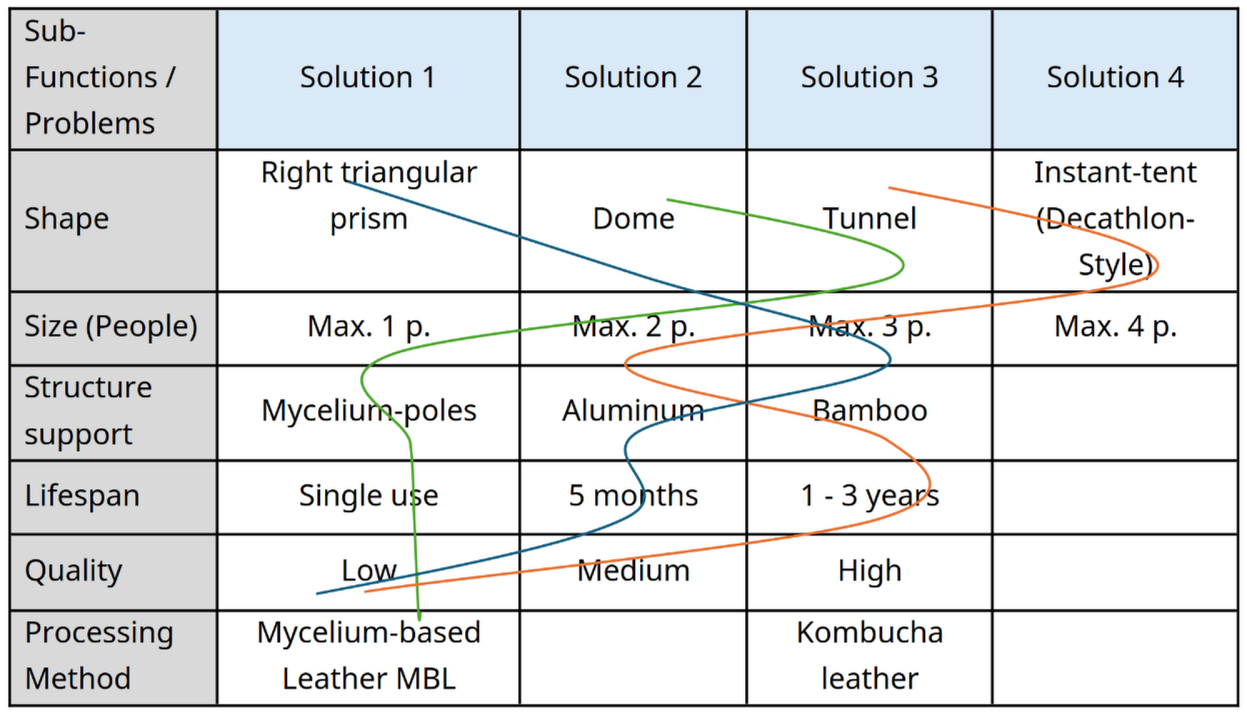
\includegraphics[width=.7\textwidth]{media/morph_box.png}
    \label{tab:morph_box}
\end{table}

\subsubsection{Description of the three solution variants}
\pph{\color{newgreen}{Variant 1: Dome tent (Single use, Fully biodegradable)}}
The first variant is a dome-shaped tent, constructed entirely from biodegradable materials,
including mycelium poles and Mycelium-Based Leather (MBL). This variant is designed for
single-use and aims to provide the highest possible grade of biodegradability. It is
produced with a focus on low-cost and low-quality materials, suitable for short-term use
at festivals.

\pph{\color{neworange}{Variant 2: Tunner tent (Four-person, Long-lasting)}}
The second variant is a tunnel tent, chosen for its optimal space-to-weight ratio, making
it suitable for accommodating four people—the largest capacity in this selection. It is
designed with higher-quality materials for a lifespan of one to three years, supported by
an aluminum structure for enhanced durability and stability.

\pph{\color{newblue}{Variant 3: Triangular prism tent (Two-person, Medium-lasting)}}
The third variant is a right triangular prism-shaped tent, designed for two people.
This option combines features from both the high-quality tunnel tent and the single-use
dome tent. It uses bamboo poles, which provide greater longevity than mycelium but are
less durable than aluminum, while still maintaining biodegradability.

The final selection between these three variants will be made in the following chapter.

\subsection{Value-Benefit analysis}
\autoref{tab:val-ben} presents the Value-Benefit analysis of the three previously described tent
variants. In alignment with our primary objective of addressing plastic waste at festivals,
biodegradability is assigned the highest priority. The affordability of each variant is
also crucial, as it must remain competitive with existing products that contribute to the
plastic waste problem. Given that the target market is festival-goers seeking short-term,
disposable solutions, the overall quality and lifespan of the tents are less critical, as
we do not aim to compete in the high-quality tent market.

The analysis includes a row for ``Weather Resistance'', which evaluates the tent's ability
to endure adverse weather conditions, such as heavy winds. This aspect is particularly
relevant as different shapes provide varying levels of structural resilience.

\subsubsection{Justified choice}
Based on the weighted ratings derived from the Value-Benefit analysis \autoref{tab:val-ben},
the Dome Tent variant emerges as the most suitable option, achieving a
total score of 680 points, the highest among all variants. This reflects its strong
alignment with customer requirements, such as affordability, ease of use, and
reduced environmental impact, making it particularly appealing to festival-
goers. Its features address the key customer demand for a sustainable,
temporary shelter while effectively contributing to the goal of reducing plastic
waste in festival environments.

\begin{table}[ht!]
    \centering
    \caption{Value-Benefit analysis}
    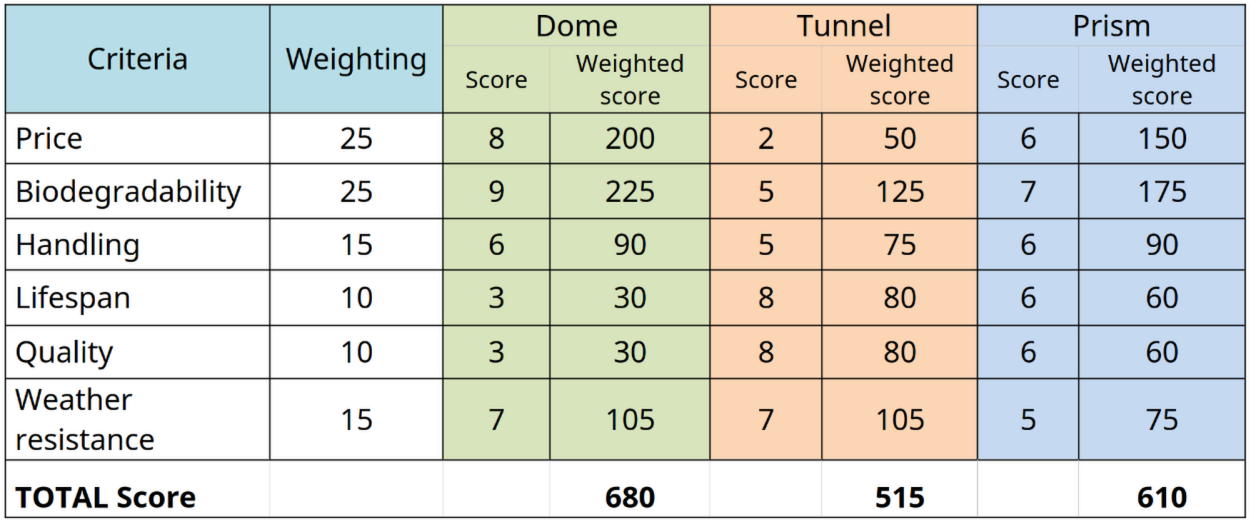
\includegraphics[width=.75\textwidth]{media/val-ben.png}
    \label{tab:val-ben}
\end{table}

\section{Final concept}

\subsection{Product concept}

\subsection{Technical specifications}

\subsection{Construction plans}

\subsection{Mock-up}
The mock-up presentation is a key part of the project, allowing users to visualize and
understand the tent's design. The tent's features, including the removable cap and door
operation with the respective materials used to create the mock-up, will be shown below.

\subsubsection{Concept of mock-up}
The \myc\ features a fully enclosed body with an upper ventilation opening, protected by a
mosquito net and rain cover (\autoref{fig:final_mockup}).\\
External poles ensure airflow and prevent water ingress. The entry is secured with a
loop-and-toggle system, and the overlapping door design blocks rain.

Made from mycelium (\autoref{fig:compact_myc}), a natural material grown from mushrooms,
it is fully recyclable and, in the worst case, mostly biodegradable. Even if abandoned,
the \myc\ minimizes environmental impact.

\newpage
\subsubsection{Final mock-up}
\begin{figure}[ht!]
    \centering
    \begin{minipage}{0.45\textwidth}
        \centering
        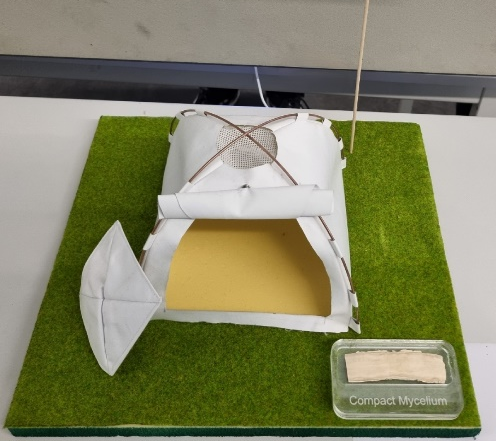
\includegraphics[width=.8\textwidth]{media/final_mockup.png}
        \label{fig:final_mockup}
        \caption{Final mock-up}
    \end{minipage}%
    \hfill
    \begin{minipage}{0.45\textwidth}
        \centering
        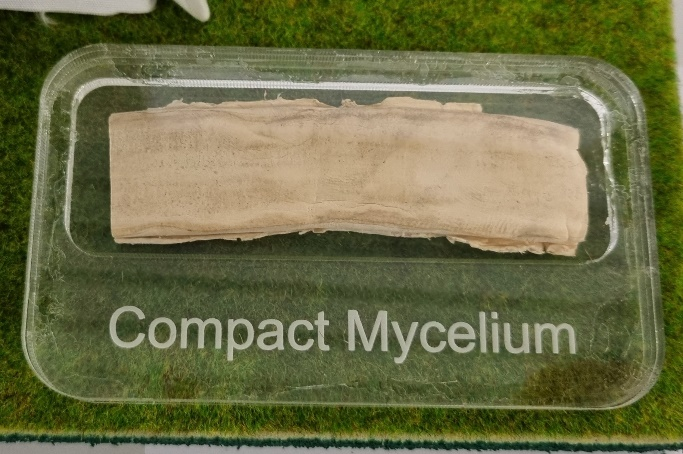
\includegraphics[width=\textwidth]{media/compact_myc.png}
        \label{fig:compact_myc}
        \caption{Compact mycelium}
    \end{minipage}
\end{figure}

\subsubsection{Technical drawing}
\begin{figure}[ht!]
    \centering
    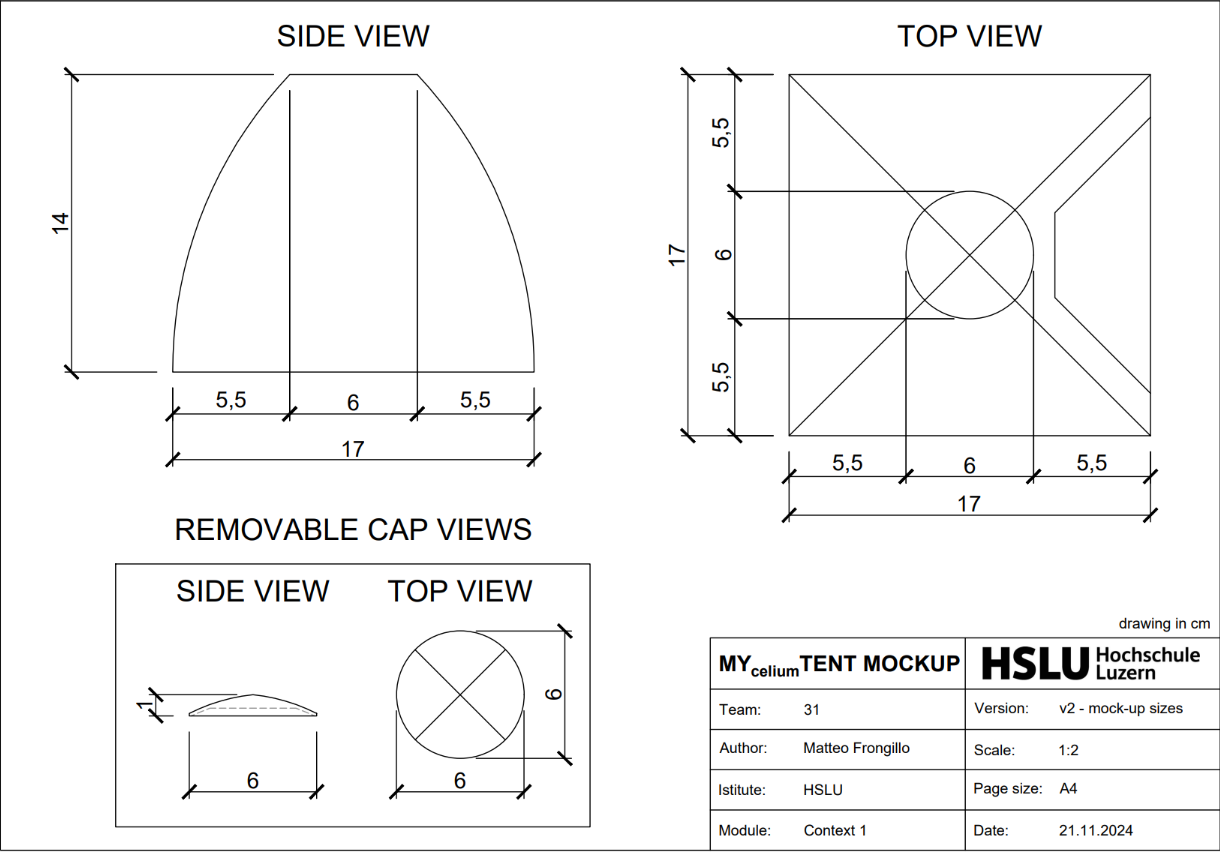
\includegraphics[width=\textwidth]{media/tent_plane.png}
    \label{fig:tent_plan}
    \caption{Technical drawing of the mock-up}
\end{figure}

\section{Testing}
This chapter examines the testing phase, which is critical to ensuring that the product
meets technical specifications and fulfils customer requirements. The expected results are
then evaluated in order to give clarification, if further tests or development is necessary.

\subsection{Tests}
The testing process is divided into two principal areas: Verification and Validation.
For each area, three different tests will be conducted.

\subsubsection{Verification}
This subchapter discusses the verification process during the testing phase. The purpose
of this process is to ensure that the product has been developed correctly and meets the
predefined requirements. Three of the most significant tests are outlined in 
\autoref{tab:verification}, with the numbers in brackets indicating the
corresponding links to the requirements catalogue, which can be found in the appendix.

\renewcommand{\arraystretch}{1.5}

\begin{table}[ht!]
    \caption{Verification tests}
    \label{tab:verification}
    \begin{tabularx}{\textwidth}{|p{2.5cm}|p{3.5cm}|p{6cm}|X|}
    \hline
    \textbf{Function} & \textbf{Requirement} & \textbf{Test procedure} & \textbf{Expected Result} \\
    \hline
    Hydrostatic head (1 / 12) & 
    The tent should have a minimum hydrostatic head of 1500 mm & 
    The hydrostatic head is determined by a water pressure test. The material is subjected to increasing water pressure. This continues until the material allows water to pass through. When the third drop has penetrated to the inside, the test ends. &
    The height of the water column at the point of water passage is above 1500 mm. \textcolor{newgreen}{$\Rightarrow$\textit{Fulfilled}} \\
    \hline
    Wind resistance (9) &
    The tent should be able to withstand a wind force of 50 km/h (Beaufort scale 6). &
    The tent is set up on a meadow and tested with a wind generator simulating a wind speed of 50 km/h for 30 minutes. Inside, it contains a sleeping bag, sleeping mat, and backpack with a total weight of 8 kg. The meadow has a minimum soil moisture of 40\%, reflecting conditions after rainfall. This worst-case scenario eliminates the need for additional tests, as drier conditions improve results. &
    The tent remains in place for half an hour. \textcolor{newgreen}{$\Rightarrow$\textit{Fulfilled}} \\
    \hline
    Air circulation (1) &
    It is not only the waterproofness that determines whether it stays dry inside the tent. The geometry of the tent must allow the humidity to be transported outside. &
    A humidifier is placed in the tent and switched on for 8 hours. It is set to release 50 ml of water per hour, which is roughly equivalent to a human being breathing. At the same time, the wind generator is set to 20 km/h to simulate a realistic wind situation on a large field. &
    No water collects on the tent floor after 8 hours: \textcolor{newgreen}{$\Rightarrow$\textit{Fulfilled}} \\
    \hline
    \end{tabularx}
\end{table}

\subsubsection{Validation}

\subsection{Discussion}
Regarding the verification tests, the primary source of uncertainty lies in the water
resistance of the material, particularly its water column. Existing materials with
adequate water resistance, such as alternatives to rubber seals, demonstrate that it is
feasible to produce a mycelium-based material with similar properties. However, further
testing is required to determine whether the material maintains its water resistance at
very thin wall thicknesses, which is crucial for meeting weight specifications.

Wind resistance is unlikely to pose a significant challenge due to the aerodynamic,
wind-slip shape of the tent. However, the ability to effectively manage moisture inside
the tent remains a concern. As this is a single-wall design, the construction and shape
of the tent play a critical role in facilitating ventilation. To address this, the
ventilation opening has been enlarged relative to the tent's total surface area. The
effectiveness of this design will only become clear during prototype testing.

Like the wind resistance, the validated operability and sustainability are unlikely to
cause later complications. This is due to the facts that the tent not only has a simple
structure and a construction manual as an available aid for the set-up process but is also
made predominantly out of a recyclable and biodegradable material. The overall durability
of the tent during a festival on the other hand could lead to further concern. Additional
tests during extended festivals with varying weather conditions will need to be performed
to clarify how well the tent can withstand longer and more challenging conditions.

\section{Conclusion}
The \myc\ project sought to address the critical environmental issue of waste
accumulation at festivals by developing a tent composed of a fully sustainable and
recyclable material. Mycelium, characterized by its high recyclability and cost-efficient
cultivation, has shown promise as a potential solution. However, a key challenge remains
the evaluation of its suitability as a tent material. Addressing this challenge requires
extensive research and development, which falls beyond the scope of this project.

Despite these challenges, the concept has demonstrated substantial potential. It addresses
an urgent environmental problem and offers a compelling business opportunity, particularly
as a B2B solution for festival operators. Collaborations with such stakeholders could
significantly enhance the project's impact and feasibility.

Future work should prioritize comprehensive research into the material properties of
Mycelium, followed by the production and evaluation of prototypes under realistic
conditions. This iterative development process will enable the refinement of the
product to ensure its functionality and durability. Given the significance of the problem
and the potential of the proposed solution, continuation of this project is strongly
recommended.

\section{List of tables and figures}
\listoftables

\listoffigures

\section{Declarations on the use of AI tools}
\begin{itemize}
    \item \textit{DeepL} and \textit{ChatGPT 4o} have been used as a spell-checker;\\
        \url{https://www.deepl.com/}\\
        \url{https://www.chatgpt.com/}
\end{itemize}

\setlength{\bibitemsep}{1.2\baselineskip}
\printbibliography[heading=none]

\section{Appendix}

\end{document}

